\documentclass[12pt,a4paper]{article}

\usepackage[utf8]{inputenc}
\usepackage[T1]{fontenc}
\usepackage{geometry}
\usepackage{xcolor}
\usepackage{booktabs}
\usepackage{enumitem}
\usepackage{tcolorbox}
\usepackage{fancyhdr}
\usepackage{tikz}

\geometry{margin=2cm}

\definecolor{primaryblue}{RGB}{0, 102, 204}
\definecolor{successgreen}{RGB}{40, 167, 69}
\definecolor{warningyellow}{RGB}{255, 193, 7}
\definecolor{dangerred}{RGB}{220, 53, 69}
\definecolor{lightgray}{RGB}{248, 249, 250}
\definecolor{sadblue}{RGB}{100, 149, 237}

\tcbuselibrary{skins, breakable}

\newtcolorbox{madbox}{
    colback=dangerred!10,
    colframe=dangerred,
    title=\textbf{MAD -- Frustrating Issues},
    fonttitle=\bfseries,
    breakable
}

\newtcolorbox{sadbox}{
    colback=sadblue!10,
    colframe=sadblue,
    title=\textbf{SAD -- Disappointing but Manageable},
    fonttitle=\bfseries,
    breakable
}

\newtcolorbox{gladbox}{
    colback=successgreen!10,
    colframe=successgreen,
    title=\textbf{GLAD -- Positive Experiences},
    fonttitle=\bfseries,
    breakable
}

\newtcolorbox{actionbox}{
    colback=primaryblue!10,
    colframe=primaryblue,
    title=\textbf{Action Items},
    fonttitle=\bfseries,
    breakable
}

\pagestyle{fancy}
\fancyhf{}
\fancyhead[L]{\textbf{Sprint Retrospective}}
\fancyhead[R]{CS2113}
\fancyfoot[C]{\thepage}

\title{
    \textbf{Sprint Retrospective}\\
    \large Template\\[0.5cm]
    \normalsize CS2113 -- Software Development Project
}
\author{[Team Name]}
\date{Sprint \_\_\_ | \today}

\begin{document}

\maketitle

%============================================================
\section{Retrospective Information}
%============================================================

\begin{tabular}{ll}
\toprule
\textbf{Sprint Number:} & \\
\textbf{Date:} & \\
\textbf{Facilitator:} & \\
\textbf{Participants:} & \\
\bottomrule
\end{tabular}

%============================================================
\section{Mad, Sad, Glad}
%============================================================

\begin{madbox}
\textit{Issues that deeply frustrated the team and prevented optimal performance}

\vspace{0.5cm}

\begin{enumerate}
    \item \hrulefill
    \item \hrulefill
    \item \hrulefill
    \item \hrulefill
    \item \hrulefill
\end{enumerate}
\end{madbox}

\vspace{0.5cm}

\begin{sadbox}
\textit{Issues that were disappointing but manageable}

\vspace{0.5cm}

\begin{enumerate}
    \item \hrulefill
    \item \hrulefill
    \item \hrulefill
    \item \hrulefill
    \item \hrulefill
\end{enumerate}
\end{sadbox}

\vspace{0.5cm}

\begin{gladbox}
\textit{Positive experiences we want to continue}

\vspace{0.5cm}

\begin{enumerate}
    \item \hrulefill
    \item \hrulefill
    \item \hrulefill
    \item \hrulefill
    \item \hrulefill
\end{enumerate}
\end{gladbox}

%============================================================
\section{Discussion Summary}
%============================================================

\subsection{What Went Well?}
\begin{itemize}
    \item[$\checkmark$]
    \item[$\checkmark$]
    \item[$\checkmark$]
\end{itemize}

\subsection{What Didn't Go Well?}
\begin{itemize}
    \item[$\times$]
    \item[$\times$]
    \item[$\times$]
\end{itemize}

\subsection{What Can We Improve?}
\begin{itemize}
    \item[$\rightarrow$]
    \item[$\rightarrow$]
    \item[$\rightarrow$]
\end{itemize}

%============================================================
\section{Action Items}
%============================================================

\begin{actionbox}
\textit{Concrete actions to implement in the next sprint}

\vspace{0.3cm}

\begin{tabular}{clll}
\toprule
\textbf{\#} & \textbf{Action} & \textbf{Owner} & \textbf{Due Date} \\
\midrule
1 & & & \\[0.5cm]
\hline
2 & & & \\[0.5cm]
\hline
3 & & & \\[0.5cm]
\hline
4 & & & \\[0.5cm]
\hline
5 & & & \\[0.5cm]
\bottomrule
\end{tabular}
\end{actionbox}

%============================================================
\section{Comparison with Previous Retrospective}
%============================================================

\subsection{Previous Action Items Status}
\begin{tabular}{clc}
\toprule
\textbf{\#} & \textbf{Action from Previous Sprint} & \textbf{Status} \\
\midrule
1 & & $\square$ Done / $\square$ In Progress / $\square$ Not Started \\
2 & & $\square$ Done / $\square$ In Progress / $\square$ Not Started \\
3 & & $\square$ Done / $\square$ In Progress / $\square$ Not Started \\
\bottomrule
\end{tabular}

\subsection{Recurring Issues}
\textit{Are there any issues that appeared in both this and the previous retrospective?}

\vspace{1cm}
\hrulefill

\hrulefill

\hrulefill

%============================================================
\section{Team Mood}
%============================================================

Rate the overall team mood for this sprint (1-5):

\begin{center}
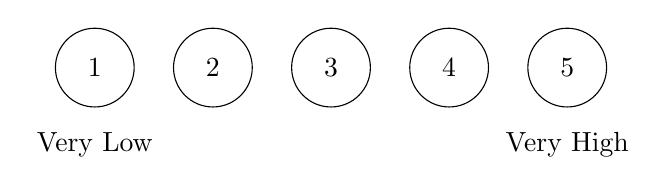
\begin{tikzpicture}
    \foreach \i in {1,...,5} {
        \node[circle, draw, minimum size=1cm] at (\i*1.5, 0) {\i};
    }
    \node[below] at (1.5, -0.7) {Very Low};
    \node[below] at (7.5, -0.7) {Very High};
\end{tikzpicture}
\end{center}

\textbf{Comments on team mood:}

\hrulefill

\hrulefill

%============================================================
\section{Notes}
%============================================================

\vspace{3cm}

%============================================================
\section{Next Steps}
%============================================================

\begin{itemize}
    \item[$\square$] Share retrospective summary with team
    \item[$\square$] Add action items to Sprint Backlog
    \item[$\square$] Update README.md with Flinga board link
    \item[$\square$] Follow up on action items during Daily Scrums
\end{itemize}

\end{document}
